% section 1 Introduction
\subsection{Background}
Although the production of ultra-high magnetic fields above several tens of Tesla has been achieved these years\cite{1_1_1},
shielding of such high fields of Tesla order still remains a challenge.
Magnetic field shielding systems are generally implemented by using ferromagnets, such as Cobalt and Ferrite.
However, the magnetic flux desity of such ferromagnets becomes saturated around several hundreds mT,
causing them unavailable of shielding Tesla order fields.
Another magnetic shielding system commonly used in MRI systems generates inversed field actively to shield the original field.
While this system is feasible on shielding magnetic fields up to several Tesla,
since it is active, extra power supply is needed and the energy consumption would be enormous.
To expand the potential of high magnetic field applications,
a passive shielding system capable of shielding high magnetic fields is required.
But first, in order to clarify constraints and design principles,
we have targeted the field generated in Space Radiation Superconducting Shields(SR2S) and dedicated to develope a high magnetic field adaptable shielding system for such scheme.

To reduce the risk of exposure induced cancer for astronauts participating in International Space Station or other space missions,
attempts to use high magnetic fields to prevent the space radiation have been conducted.
The concept is similar to the geomagnetism from the Earth,
which generates a high magnetic field from the north or the south pole to divert the cosmic ray coming from deep space by the Lorentz force.
A schematic diagram is shown in Fig. \ref{fig:SR2S}.
The concept is quite straightforward,
and the magnitude of the magnetic field needed to shield the cosmic ray has been studied by multiple projects.
Many of them have reported a result of 1$\sim$8T magnetic field being generated around the spacecraft \cite{1_1_2}$\sim$\cite{1_1_5}.
In such condition, a magnetic field shielding system would be required to prevent the strong field penetrating into the spacecraft
causing unintentional side effects on human bodies and electrical equipments.
Moreover, the disturbance of the external fields should be taken into consideration as well.
In SR2S, the external strong field is used to divert cosmic rays and shouldn't be weakened by the magneitc field shielding system.
The property not to disturb external field is more widely required rather than only occurs in the SR2S case.
For instance, in the case of MRI, the strong field is used to conduct delicate medical investigation,
and thus the stability and homogeneity of which should be considered the first priority.
Since external high fields to be shielded are often producted intentionally for specific application reasons,
minimum disturbance of external fields is required for any high field shielding system.
\begin{figure}[H]
  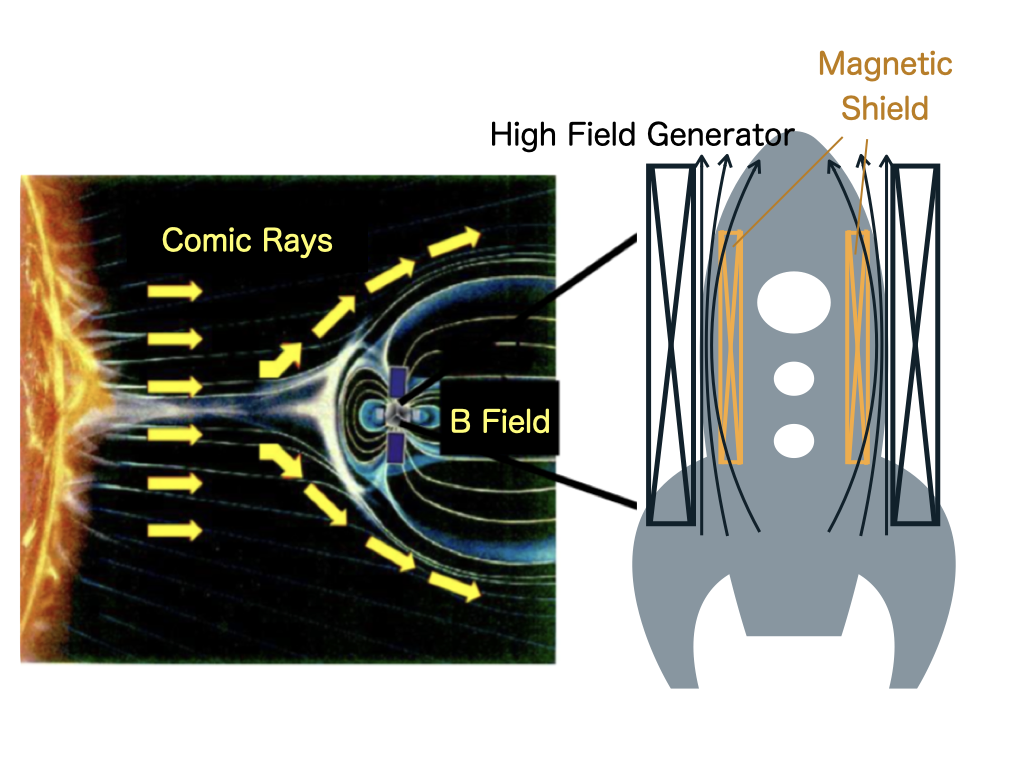
\includegraphics[width=18cm, bb=9 9 900 700]{./section1Introduction/solar.png}
  \caption{A schematic diagram of the comic ray shielding system and targeted magnetic field shielding system. }
  \label{fig:SR2S}
\end{figure}
\begin{figure}[H]
  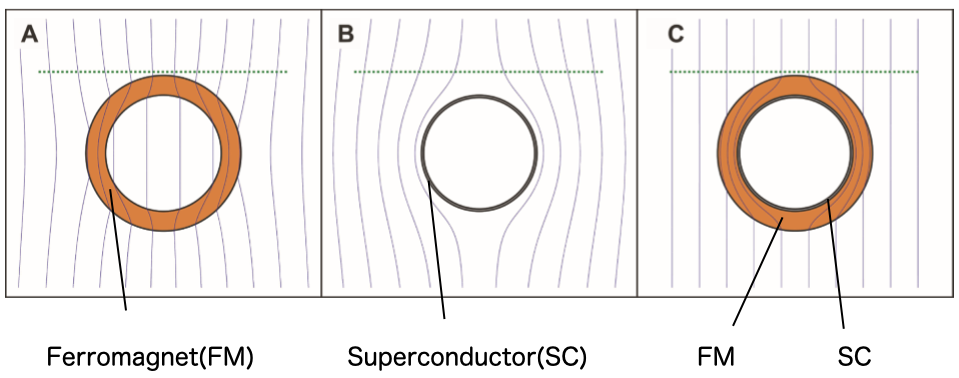
\includegraphics[width=18cm, bb=9 9 900 350]{./section1Introduction/cloak.png}
  \caption{The magnetic flux distribution when (A) a magnet, (B) a superconductor ring and (C) a manetic cloak is placed in a stable magnetic field.}
  \label{fig:cloak}
\end{figure}

In order to achieve the goal of shielding high magnetic field while not disturbing external fields,
we have introduced a new shielding system of which the concept comes from the magnetic cloak proposed by Fedor G. et al.\cite{1_1_6}.
A magnetic cloak consists of superconductor and ferromagnet in a double-layered cylindrer shape.
Generally, a ferromagnet has the property of attracting the magnetic flux while a superconductor owns the property of excluding the magnetic flux, the so called diamagnetism.
Fedor has shown that by combining the two materials which have the opposite effects,
eliminating the internal magnetic flux while not altering external fields can be achieved simultaneously.
This property is called "cloak" on magnetic fields, the concept is shown in Fig. \ref{fig:cloak}.
However, since the model relies on the Meissner effect to exclude to magnetic flux,
adaption on high magnetic fields is infeasible.
In fact, in Fedor's pape, it has been claimed to be effective up to 40 mT, which is far beyond the goal of shielding fields in several Tesla level.


In contrast, we took the idea of combining superconductors and ferromagnets and reform the construction to develope a passive magnetic cloak
which is suitable for shielding high magnetic fields on several Tesla level,
with expected scalability to further more.
In this thesis, the studies of the effectiveness and the optimized construction of the new magnetic cloak would be denoted
from various perspectives carried out by simulation and experiments.

\newpage
\subsection{High Magnetic Fields in Space Radiation Superconducting Shields}
The risk from space radiation exposure is an important concern for astronauts participating in International Space Station(ISS) missions.
Recently it has been reported that astronauts participated in at least 1 year ISS missions near solar minimum risk several percent exposure induced cancer.
For the sake of space advancement, shielding equipments of comic rays are required.

To prevent the penetration of the comic rays, many researches have been conducted.
The concept is similar to the geomagnetism from the Earth,
which generates a strong magnetic field from the North pole, covering the whole atmosphere.
Since most of the comic rays are positive charges, they tend to roll along the magnetic flux due to the Lorentz force, $F = v\times B$.
This infers that if the magnetic field is strong enough and placed properly,
it is able to divert the comic ray and work as a radiation shielding equipment.

Several projects have been set up to reproduce this mechanism on a spacecraft.
Many of them have reported a result of generating magnetic field among $1\sim8$ T on the surroundings \cite{1_1_2}$\sim$\cite{1_1_5}.
To make the system clear, a schematic diagram of the equipment is represented in Fig. \ref{fig:SR2SwithoutShielding}.
A high magnetic field of several Tesla generated along the long axis of the spacecraft spreads into the open space,
forming a magnetic wall to stop the comic ray from penetraing.
Although this system is said to be working well on diverting radiation, some magnetic shielding system is needed to protect electrical equipments from exposure of the high field.
In our research, rather than recalculate parameters or doing further studies of the comic ray shielding system,
we have left the detail of it unvarified and focused on developing a magnetic field shielding system suitable for this scheme.
\begin{figure}[H]
  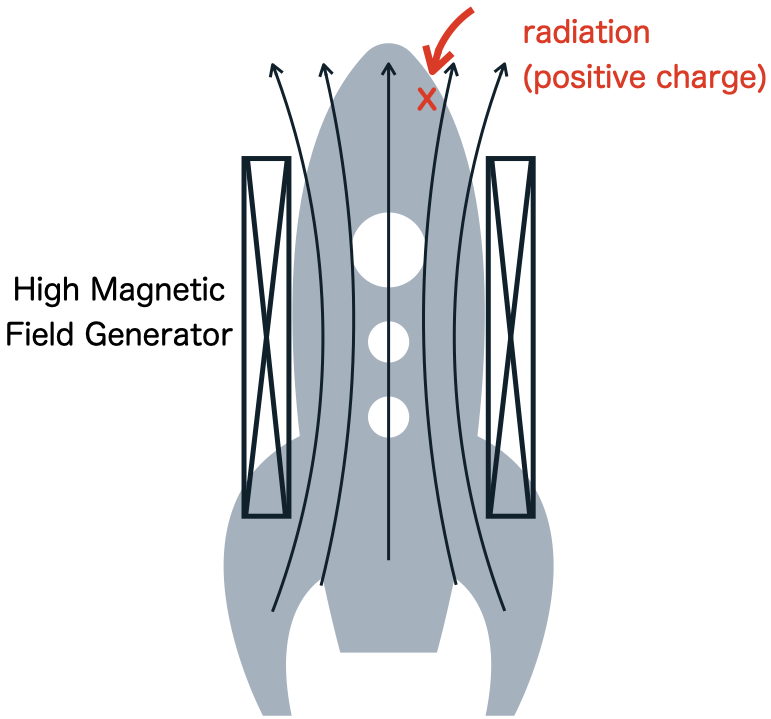
\includegraphics[width=18cm, bb=9 9 900 900]{./section1Introduction/SR2SwithoutShielding.png}
  \caption{A schematic diagram of the  comic ray shielding system using high magnetic fields. }
  \label{fig:SR2SwithoutShielding}
\end{figure}


\newpage
\subsection{Difficulties of Shielding High Magnetic Fields}
The conventional method used in magnetic shielding is using ferromagnets,
which are known to have a strong relative permeability of 1000 to several hundreds of thousand.
When imposed by some external field, magnetization $M$ with almost opposite direction against $H$ field will be induced.
With such high permeability, induced magnetization in ferromagnet becomes the dominant term in $B = \mu H + M$,
causing the $B$ field to divert significantly in the surroundings of the magnet.

Consider a hollow cylinder placed in a stable uniform field, shown in Fig. \ref{fig:FM}.
\begin{figure}[H]
  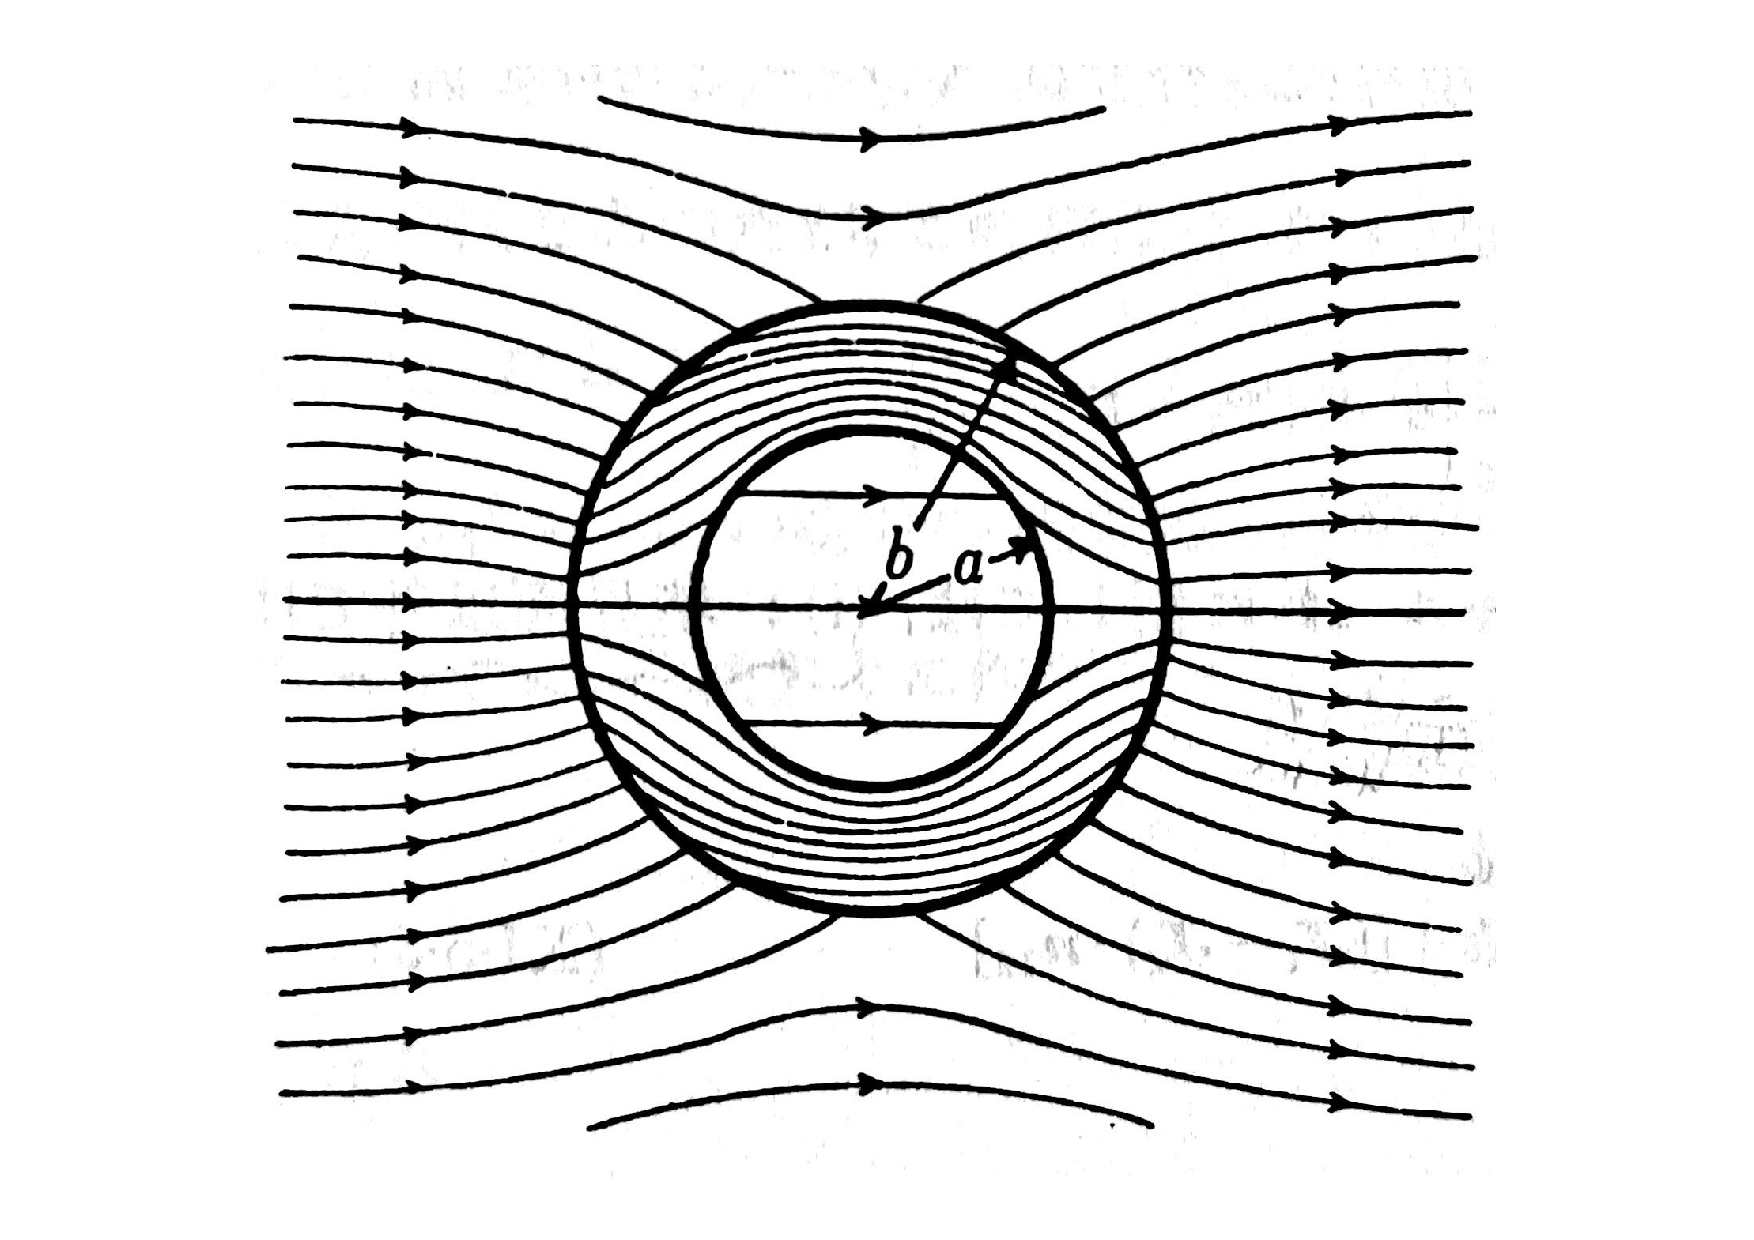
\includegraphics[width=18cm, bb=9 9 900 600]{./section1Introduction/FM.pdf}
  \caption{The $B$ field distribution near the cylinder placed in an uniform stable field \cite{1_1_7}.}
  \label{fig:FM}
\end{figure}
\begin{table}[H]
  \centering
  \caption{Shielding effects under various magnet thickness(a/b) and relative permeability($\mu_r$).}
  \label{tab:FM}
  \begin{tabular}{cc|rrrrr}\hline\hline
    a/b &  & 0.99 & 0.8 & 0.6 & 0.4 & 0.2\\\hline
    $H_{internal}/H_{external}$ & $\mu_r = 100$ & 3/5 & 1/12 & 1/18 & 1/22 & 1/23 \\
    $H_{internal}/H_{external}$ & $\mu_r = 1000$ & 3/23 & 1/109 & 1/175 & 1/209 & 1/221 \\\hline\hline
  \end{tabular}
\end{table}
Affected by the induced magnetization $M$, the magnetic flux in the magnet part is reinforced and that in the internal space is reduced.
The internal field is shown in detail in Tab. \ref{tab:FM}, along with different permeability.
From Tab. \ref{tab:FM},
increasing the permeability or the thickness of the magnet yields a better shielding effect.
As well, elimination near 99\% in the interior space can be achieved using magnets with relative permeability of several thousands,
which is a common value for modern ferromagnetic materials.
This method is often known as the "magnetic screening".

Due to its simplicity, magnetic screening is widely used in industry, especially in electrical devices like smartphone.
However, common ferromagnetic materials like ferrite can only provide a limited magnetization up to 700 mT,
making the magnetic screening to fail on high imposed fields as several Tesla level.
This is the main difficulty on high magnetic field shielding.

Besides, since the generation of high magnetic fields itself is difficult, they are often produced intentionally for application reasons.
In SR2S they are applied to prevent comic rays, in MRI they are used to conduct detailed examination of human bodies,
in biological or physical regions they surves as a means of trigger of new phenomena, etc.
When a magnetic shielding system is inserted in the neighborhood of these high fields,
those fields may be disturbed.
In Fig. \ref{fig:cloak}(A), it is clear that the field near the ferromagnet is disturbed due to the induced magnetization.
In Fig. \ref{fig:cloak}(B), disturbance on the external field due to the diamagnetism of the superconductor can also be observed.
Consider the application of these fields, the stability of which should be given the first priority and thus
the property that magnetic shielding systems implemented afterwards not altering the external field is required.
In spite of such demand, conventional shielding methods fail to meet the needs, leaving it an open challenge.

As describe in section 1.1, the property that internal field is eliminated while the external field distribution remains unchanged
is known as "cloak" on magnetic fields.
This concept has started to become possible theese years using anisotropic, spatially inhomogeneous, or singular values of magnetic permeability \cite{1_1_8}$\sim$\cite{1_1_11}.
A further simplified model has been proposed in Fedor's paper \cite{1_1_6} in 2012, in which ferrormagnets and low-temperature superconductors are used.


However, all of them are neither designed for high magnetic field application,
nor capable to shield fields of several Tesla.
With high magnetic field application grow,
a magnetic cloak capable fo operating in high field is required.
To achieve such system, the problem of magnetization saturation under high fields should be overcame
while disturbance of the external field is eliminated,
which seems extremely difficult.


\newpage
\subsection{Purpose of the Study}
To expand the potential application of high magnetic fields of several Tesla,
a magnetic cloak adaptable to high fields is required.
In detail, the cloak must satisfy 2 properties:
\begin{enumerate}
  \item Able to shield magnetic fields of several Tesla.
  \item Have a limited disturbance on external fields.
\end{enumerate}

In this study, in order to clarify the constraints and real-world application,
we have focused on the SR2S project in space usage,
and set up the goal to be the followings, which is slightly different from the above:
\begin{enumerate}
  \item Able to shield 1 T magnetic field.
  \item Have a limited weakening effect on the external field.
\end{enumerate}
For the 1st property, we have taken into consideration the equipment in our laboratory.
Since the S2RS project generates $1\sim 8$T fields and the ferromagnet applied in this study owns a saturation field of 700 mT,
this setting is considered sufficient to testify the proposed magnetic cloak.
For the 2nd property, since the magnetic field in the SR2S project is used to divert the comic ray,
the external field being weakened should be consider a larger issue than being reinforced.
A weakened area of the external field will allow the comic rays penetrating into the spacecraft causing potnetial damage on human bodies while a strengthened area of the external field will not trigger any fatal problem.
For convinience, we have changed the 2nd property to be concentrated in preventing the external field from weakening.

Through this thesis, a new designed magnetic cloak suitable to work in high fields will be introduced,
with which the effectiveness and optimal construction will be described further in the following sections.


\newpage
\subsection{Construction of This Thesis}
In section 2, we first describe our proposal of overcoming the difficulties of shielding high magnetic fields.
The concept, construction, how it works along with the improvement from the conventional magnetic cloak are denoted.

In section 3, the evidence on the expectable capability of achieving cloak on high magnetic fields are shown.
To proof the ability of shielding effect,
we have conducted a series of experiments on the scaled down model.
Since each of the experiment have been designed for specific purpose,
the theory, experimental set up, results and discussion are described relatively.

In section 4, after the effectiveness have been revealed, the optimized construction of the position of superconductor tapes and ferromagnets are stated with detailed simulation.
The simulation are conducted by advance methods such as the Finite Element method and modern optimization algorithms which might be unfamiliar to readers who don't have a background on algorithm region.
Despite that the full detail of theese analysis is beyond the scope of this thesis,
we have been dedicated in explaining the story step by step with information described as detailed as possible.
If it is found difficult to under stand, please refer to the articles in reference.

In section 5, the result done on 1 T environment using the model near full scale is stated and discussed.
Finally, the whole thesis is summaried in section 6.


\newpage
\begin{thebibliography}{11}
  \bibitem{1_1_1} N. Miura, T. Goto, K. Nakao, S. Takeyama, T. Sakakibara, T. Haruyama, T. Kikuchi, "Production of ultra-high magnetic fields and their application to solid state physics", Physica B: Condensed Matter, Volume 155, Issues 1–3, Pages 23-32 (1989)
  \bibitem{1_1_2} Filippo Ambroglini1, Roberto Battiston2 and William J. Burger, "Evaluation of Superconducting Magnet Shield Configurations for Long Duration Manned Space Missions", Frontiers in Oncology, Vol. 6, p. 97 (2016)
  \bibitem{1_1_3} R. Musenich, V. Calvelli, S. Farinon, W. J. Burger, R. Battiston, "Space Radiation Superconducting Shields", Journal of Physics: Conference Series 507 032033 (2014)
  \bibitem{1_1_4} Westover SC, Meinke RB, Battiston R, Burger WJ, Van Sciver S, Washburn S, et al. Magnet Architectures and Active Radiation Shield Study. NASA Institute for Advanced Concepts (NIAC) Phase 1 Final Report (2012)
  \bibitem{1_1_5} Battiston R, Burger WJ, Calvelli V, Musenich R, Choutko V, Datskov VI, et al. Superconductive Magnet for Radiation Shielding of Human Spacecraft. (2011)
  \bibitem{1_1_6} Fedor Gömöry et al., "Experimental Realization of a Magnetic Cloak", Science 335, 1466 (2012)
  \bibitem{1_1_7} 竹山 説三, "電磁気學現象理論", p. 269, 丸善 (1949)
  \bibitem{1_1_8} 1. J. B. Pendry, D. Schurig, D. R. Smith, Science 312, 1780 (2006)
  \bibitem{1_1_9} U. Leonhardt, Science 312, 1777 (2006)
  \bibitem{1_1_10} A. Greenleaf, M. Lassas, G. Uhlmann, Physiol. Meas. 24, 413 (2003)
  \bibitem{1_1_11} A. Alù, N. Engheta, J. Opt. A Pure Appl. Opt. 10, 093002 (2008)
\end{thebibliography}
